\section{سوال چهارم - تئوری}

یکی از مشکلات ترنسفورمرها مرتبه هزینه محاسباتی و هزینه ذخیره‌سازی عملیات \lr{self-attention} است که از مرتبه $O(N^2)$ می‌باشد. تلاش‌هایی برای کاهش این مشکل انجام شد. مقالاتی نشان دادند که عملکرد \lr{softmax} باعث می‌شود تا نتوانیم این پیچیدگی را کاهش دهیم. توضیح دهید چرا عملکرد \lr{softmax} باعث وجود این مسئله می‌شود. همچنین یکی از پیشنهادها برای حل این مشکل استفاده از مکانیزم‌های توجه کرنلی است. در مورد این مکانیزم تحقیق کنید و نشان دهید چطور این روش منجر به کاهش پیچیدگی می‌شود. یک کرنل به دلخواه انتخاب کنید و عبارت «۱» را بازنویسی کنید و مرتبه زمانی و حافظه مورد نیاز برای عملکرد \lr{self-attention} را محاسبه کنید. لطفا به مقاله که برای انتخاب کرنل مراجعه کردید، ارجاع دهید.

\begin{equation}
	Attention(Q, K, V)=softmax(\frac{QK^T}{\sqrt{d_k}})V
\end{equation}




\begin{qsolve}
بر اساس رابطه ۱ مکانیزم \lr{Self-attention}  شامل محاسبه ضرب داخلی $Q$و $K$ می‌شود که منجر به تولید ماتریسی با ابعاد $N\times N$ می‌شود. تابع \lr{softmax} به هر سطر این ماتریس اعمال می‌شود که مقادیر توجه را نرمالیزه می‌کند. پیچیدگی درجه دوم از اینجا ناشی می‌شود که:

\begin{enumerate}
	\item \textbf{ضرب ماتریسی}: محاسبه \( QK^T \) شامل عملیات \( O(N^2d_k) \) است.
	\item \textbf{محاسبه \lr{softmax}}: اگرچه softmax برای هر سطر \( O(N) \) است، به همه \( N \) سطر اعمال می‌شود که منجر به \( O(N^2) \) در کل می‌شود.
\end{enumerate}

برای حل مشکل پیچیدگی درجه دوم، مکانیزم‌های توجه مبتنی بر هسته پیشنهاد شده‌اند. این روش‌ها با استفاده از توابع هسته، تابع \lr{softmax} را تقریب می‌زنند که می‌تواند پیچیدگی محاسبات توجه را کاهش دهد.

یکی از این روش‌ها استفاده از نقشه ویژگی تصادفی برای تقریب تابع هسته \lr{softmax} است. ایده اصلی این است که ورودی را با استفاده از نقشه ویژگی به فضایی تبدیل کنیم که در آن ضرب داخلی، تقریب تابع هسته اصلی را ارائه دهد. حال سوال پیش می‌آید که از چه هسته هایی می‌توان استفاده نمود؟

\begin{enumerate}
	\item \textbf{هسته \lr{RBF}}\\
هسته \lr{RBF} یکی از انتخاب‌های محبوب برای چنین تقریب‌هایی است. هسته \lr{RBF} به صورت زیر تعریف می‌شود:
	
	\[ k(x, y) = e^{-\frac{\|x - y\|^2}{2\sigma^2}} \]
	
اما برای کارایی محاسباتی، می‌توانیم از تقریب های سری فوریه تصادفی استفاده کنیم.


	\item \textbf{تقریب \lr{softmax} با هسته \lr{RBF}}\\
	هسته \lr{RBF} می‌تواند با استفاده از ویژگی‌های سری فوریه تصادفی به صورت زیر تقریب زده شود:
	
	\[ k(x, y) \approx \phi(x)^T \phi(y) \]
	
	که در آن \( \phi(x) \) یک نقشه ویژگی تصادفی از \( x \) است.
\end{enumerate}
\end{qsolve}






\begin{qsolve}
	\begin{enumerate}
		
		
			\item \textbf{بازنویسی توجه مبتنی بر هسته}\\
			با استفاده از این تقریب، مکانیزم توجه می‌تواند به صورت زیر بازنویسی شود:
			
			\[ Attention(Q, K, V) \approx \left(\phi(Q) \phi(K)^T \right) V \]
		
		
		
		
			\item \textbf{کاهش پیچیدگی}\\
			\begin{itemize}
					\item \textbf{تبدیلات}: نقشه ویژگی تصادفی \( \phi \) به طور معمول ابعاد کمتری \( r \) دارد. تبدیل \( Q \) و \( K \) به \( \phi(Q) \) و \( \phi(K) \) به ترتیب شامل عملیات \( O(Nd_kr) \) است.
					\item \textbf{ضرب داخلی}: ضرب داخلی \( \phi(Q) \phi(K)^T \) شامل عملیات \( O(N^2 r) \) است.
					\item \textbf{ضرب نهایی با \( V \)}: ضرب نتیجه با \( V \) شامل عملیات \( O(Nrd_v) \) است.
				\end{itemize}
			با انتخاب \( r \ll N \)، پیچیدگی به طور قابل توجهی کاهش می‌یابد.
		
		
		
		
		
		
		\item \textbf{پیچیدگی زمانی و حافظه}\\
		\begin{itemize}
			\item \textbf{پیچیدگی زمانی}:
			\begin{itemize}
				\item نقشه ویژگی: \( O(Nd_kr) \)
				\item ضرب داخلی: \( O(N^2r) \)
				\item محصول نهایی: \( O(Nrd_v) \)
			\end{itemize}
			
			با ترکیب اینها، پیچیدگی زمانی کلی:
			
			\[ O(Nd_kr + N^2r + Nrd_v) \]
			
			با \( r \ll N \)، عبارت غالب \( O(N^2r) \) است.
			
			\item \textbf{پیچیدگی حافظه}:
			\begin{itemize}
				\item ذخیره \( \phi(Q) \) و \( \phi(K) \): \( O(Nr) \)
			\end{itemize}
		\end{itemize}
		
		
		
	\end{enumerate}
\end{qsolve}


\begin{latin}
	\begin{thebibliography}{9}
		\bibitem{ref1}
		"Rethinking Attention with Performers" by Choromanski et al. (2021), which introduces the Performer model using kernel-based approximations to reduce the complexity of self-attention.
	\end{thebibliography} 
\end{latin}









%مدل‌های مولد حوزه‌ی تصویر به چهارچوب‌های مختلف تقسیم می‌شوند. وجه مشترک همه‌ی این مدل‌ها این است که تلاش می‌کنند تا با یادگیری توزیع داده‌ها نمونه‌های جدیدی از آن تولید کنند. تاکنون مدل‌های مولد حوزه‌ی تصویر را می‌توان در چهار قالب کلی شامل خودکدگذارهای تغییراتی\footnote{\lr{Variational Autoencoder}}، شبکه‌های مولد تقابلی، جریان‌های نرمال‌ساز\footnote{Normalizing Flows} و مدل‌های پخشی\footnote{\lr{Diffusion Models}} دسته‌بندی کرد که در هر قالب انواع مختلفی از پیاده سازی‌ها وجود دارد.
%
%\begin{enumerate}
%	\item
%در \href{https://arxiv.org/pdf/2112.07804}{\textcolor{magenta}{این مقاله}}
% سه نیازمندی کلی برای کارایی یک مدل مولد حوزه‌ی تصویر ذکر می‌شود که عبارتند از: تولید نمونه‌های با کیفیت، سرعت بالای تولید نمونه و تنوع نمونه‌های تولیدی. و نیز اشاره می‌شود که هر مدل مولدی که تاکنون در یکی از قالب‌هایی که بالاتر ذکر شد ارائه شده است در یکی از این سه نیازمندی ضعیف عمل می‌کند. با بررسی مقاله توضیح دهید که هر مدل در چه زمینه‌ای و به چه علتی ضعیف عمل می‌کند؟
%\end{enumerate}
%
%
%\begin{center}
%	\includegraphics*[width=0.4\linewidth]{pics/img3.png}
%	\captionof{figure}{مشکل سه‌گانه مدل‌های مولد}
%	\label{مشکل سه‌گانه مدل‌های مولد}
%\end{center}
%
%
%\begin{qsolve}
%	در این مقاله، ضعف‌های شبکه‌های مولد نام‌برده به‌صورت زیر بیان شده است:
%	
%	\begin{enumerate}
%		\item \textbf{شبکه \lr{GAN}:}
%		\begin{itemize}
%			\item ضعف: پوشش مُد و تنوع نمونه‌ها
%			\item دلیل: شبکه‌های \lr{GAN} به تولید نمونه‌های با کیفیت بالا و سریع معروف هستند، اما اغلب از پوشش مُد ضعیف رنج می‌برند که به آن پدیده فروپاشی مُد گفته می‌شود. این به این معناست که \lr{GAN}ها ممکن است نمونه‌های بسیار مشابهی را به طور مکرر تولید کنند و نتوانند تنوع کامل داده‌های آموزشی را به تصویر بکشند
%		\end{itemize}
%		
%		\item \textbf{\lr{VAE} ها و \lr{Normalizing Flows}:}
%		\begin{itemize}
%			\item ضعف: پوشش مود و تنوع نمونه‌ها
%		\end{itemize}
%	\end{enumerate}
%\end{qsolve}
%
%
%\begin{qsolve}
%	\begin{itemize}
%		\item دلیل: در حالی که \lr{VAEs} و جریان‌های نرمال‌ساز می‌توانند مُدهای داده را به خوبی پوشش دهند و تنوع در نمونه‌های تولید شده را تضمین کنند، اغلب نمونه‌هایی با کیفیت پایین‌تر نسبت به \lr{GAN}ها و مدل‌های انتشار تولید می‌کنند. از دست دادن بازسازی که در \lr{VAEs} استفاده می‌شود، معمولاً منجر به خروجی‌های مبهم می‌شود و جریان‌های نرمال‌ساز، در حالی که قابل برگشت و انعطاف‌پذیر هستند، می‌توانند در تولید تصاویر با \lr{fidelity} بالا نیز مشکل داشته باشند
%	\end{itemize}
%	
%	\begin{enumerate}
%		\item [3.] \textbf{مدل‌های پخشی}
%		\begin{itemize}
%			\item ضعف: سرعت نمونه‌گیری پایین
%			\item دلیل: مدل‌های انتشار قادر به تولید نمونه‌های با کیفیت بالا و متنوع هستند اما به دلیل فرآیند نمونه‌گیری آهسته خود دچار محدودیت می‌شوند. این امر به دلیل نیاز به بسیاری از مراحل نویززدایی تکراری است که هر مرحله شامل محاسبات پیچیده‌ای می‌شود. این امر آنها را از نظر محاسباتی گران و زمان‌بر می‌کند که کاربرد عملی آنها را محدود می‌کند
%		\end{itemize}
%	\end{enumerate}
%	
%این مقاله (\lr{DD-GANs}) را برای رفع این ضعف‌ها پیشنهاد می‌کند که نقاط قوت \lr{GAN}ها و مدل‌های انتشار را ترکیب می‌کند. هدف \lr{DD-GAN}ها کاهش هزینه نمونه‌گیری مدل‌های انتشار در حالی که کیفیت بالا و تنوع نمونه‌ها را حفظ می‌کنند.
%\end{qsolve}
%
%
%
%
%مدل‌های پخشی دسته‌ای از مدل‌های مولد هستند که در حال حاضر بهترین مدل تولید تصویر شناخته می‌شوند. در مدل‌های پخشی احتمالاتی از یک ذخیره‌ی مارکف برای مدل کردن فرآیند نویززدایی و نویز افزایی استفاده می‌شود و دو مسیر کلی رو به جلو\footnote{Forward} و رو به عقب\footnote{Backward} در نظر گرفته می‌شود. در مسیر رو به جلو داده‌ی اولیه مرحله به مرحله با نویز تخریب می‌شود تا به یک نویز گاوسی تبدیل شود و در فرآیند رو به عقب نیز نویز زدایی با شروع از یک نویز تصادفی اولیه انجام می‌شود تا به نمونه‌ای جدید از توزیع داده‌ها برسیم. این موضوع در تصویر «\textcolor{blue}{\ref{فرایند کلی مدل‌های پخشی}}» آورده شده است.
%
%\begin{center}
%	\includegraphics*[width=0.9\linewidth]{pics/img4.png}
%	\captionof{figure}{فرایند کلی مدل‌های پخشی}
%	\label{فرایند کلی مدل‌های پخشی}
%\end{center}
%
%
%
%
%\begin{enumerate}
%	\item
%با توجه به مقاله‌ی \href{https://arxiv.org/abs/2006.11239}{\textcolor{magenta}{مدل‌های پخشی احتمالاتی}}، در مسیر رو به جلو نیازی به اضافه کردن نویز به صورت مرحله به مرحله نیست و می‌توان نویز اضافه شونده به هر مرحله را به صورت مستقیم و با استفاده از رابطه‌ی زیر به دست آورد:
%
%	$$ q(\mathbf{x}_t | \mathbf{x}_0) = \mathcal{N}(\mathbf{x}_t ; \sqrt{\overline{\alpha}_t} \mathbf{x}_0, (1 - \overline{\alpha}_t) \mathbf{I}) $$
%
%
%با استفاده از خاصیت نویز گاوسی رابطه‌ی بالا را اثبات کنید. (\textcolor{blue}{راهنمایی:} اگر دو متغیر نرمال مستقل داشته باشیم جمع آنها نیز نرمال است.)
%
%
%\begin{qsolve}
%	
%	برای اثبات رابطه:
%	\[ 
%	q(\mathbf{x}_t | \mathbf{x}_0) = \mathcal{N}(\mathbf{x}_t ; \sqrt{\overline{\alpha}_t} \mathbf{x}_0, (1 - \overline{\alpha}_t) \mathbf{I}) 
%	\]
%	
%	باید از ویژگی نویز گوسی و ماهیت بازگشتی فرآیند انتشار استفاده کنیم.
%	
%	فرآیند انتشار به گونه‌ای تعریف می‌شود که در هر گام \( t \)، نویز به حالت قبلی \( \mathbf{x}_{t-1} \) اضافه می‌شود. به طور خاص، فرآیند پیشرو به صورت زیر است:
%	\[ 
%	q(\mathbf{x}_t | \mathbf{x}_{t-1}) = \mathcal{N}(\mathbf{x}_t ; \sqrt{\alpha_t} \mathbf{x}_{t-1}, (1 - \alpha_t) \mathbf{I}) 
%	\]
%	که در آن \( \alpha_t \) پارامتری است که میزان نویز اضافه شده در هر گام را کنترل می‌کند.
%	
%	حال اگر فرآیند را از \( \mathbf{x}_0 \) تا \( \mathbf{x}_t \) در نظر بگیریم. می‌توانیم \( \mathbf{x}_t \) را بر حسب \( \mathbf{x}_0 \) و نویز اضافه شده بنویسیم. با استفاده از ویژگی بازگشتی، داریم:
%	\[ 
%	\mathbf{x}_t = \sqrt{\alpha_t} \mathbf{x}_{t-1} + \sqrt{1 - \alpha_t} \mathbf{\epsilon}_t 
%	\]
%	که در آن \( \mathbf{\epsilon}_t \sim \mathcal{N}(0, \mathbf{I}) \) نویزی است که در گام \( t \) اضافه شده است.
%	
%	برای یافتن رابطه بین \( \mathbf{x}_t \) و \( \mathbf{x}_0 \)، \( \mathbf{x}_{t-1} \) را به‌صورت بازگشتی بسط می‌دهیم:
%	\[ 
%	\mathbf{x}_{t-1} = \sqrt{\alpha_{t-1}} \mathbf{x}_{t-2} + \sqrt{1 - \alpha_{t-1}} \mathbf{\epsilon}_{t-1} 
%	\]
%	
%	این بسط را تا \( \mathbf{x}_0 \) ادامه می‌دهیم:
%	\[ 
%	\mathbf{x}_t = \sqrt{\alpha_t} (\sqrt{\alpha_{t-1}} \mathbf{x}_{t-2} + \sqrt{1 - \alpha_{t-1}} \mathbf{\epsilon}_{t-1}) + \sqrt{1 - \alpha_t} \mathbf{\epsilon}_t 
%	\]
%	\[ 
%	= \sqrt{\alpha_t \alpha_{t-1}} \mathbf{x}_{t-2} + \sqrt{\alpha_t (1 - \alpha_{t-1})} \mathbf{\epsilon}_{t-1} + \sqrt{1 - \alpha_t} \mathbf{\epsilon}_t 
%	\]
%	
%	این روند را به صورت تکراری ادامه می‌دهیم:
%	\[ 
%	\mathbf{x}_t = \left( \prod_{s=1}^t \sqrt{\alpha_s} \right) \mathbf{x}_0 + \sum_{s=1}^t \sqrt{1 - \alpha_s} \left( \prod_{u=s+1}^t \sqrt{\alpha_u} \right) \mathbf{\epsilon}_s 
%	\]
%	
%	تعریف می‌کنیم \( \overline{\alpha}_t = \prod_{s=1}^t \alpha_s \). سپس داریم:
%	\[ 
%	\mathbf{x}_t = \sqrt{\overline{\alpha}_t} \mathbf{x}_0 + \sum_{s=1}^t \sqrt{1 - \alpha_s} \left( \prod_{u=s+1}^t \sqrt{\alpha_u} \right) \mathbf{\epsilon}_s 
%	\]
%	
%	عبارت‌های نویز \( \mathbf{\epsilon}_s \) گاوسی‌های مستقل هستند. جمع متغیرهای تصادفی گاوسی مستقل نیز گاوسی است با میانگین برابر با جمع میانگین‌های آنها و واریانس برابر با جمع واریانس‌های آنها.
%	
%	میانگین \( \mathbf{x}_t \):
%	\[ 
%	\mathbb{E}[\mathbf{x}_t] = \sqrt{\overline{\alpha}_t} \mathbf{x}_0 
%	\]
%	
%	واریانس \( \mathbf{x}_t \):
%	\[ 
%	\text{Var}(\mathbf{x}_t) = \sum_{s=1}^t (1 - \alpha_s) \left( \prod_{u=s+1}^t \alpha_u \right) = (1 - \overline{\alpha}_t) \mathbf{I} 
%	\]
%	
%	بنابراین، \( \mathbf{x}_t \) با توجه به \( \mathbf{x}_0 \) از توزیع گاوسی پیروی می‌کند:
%	\[ 
%	q(\mathbf{x}_t | \mathbf{x}_0) = \mathcal{N}(\mathbf{x}_t ; \sqrt{\overline{\alpha}_t} \mathbf{x}_0, (1 - \overline{\alpha}_t) \mathbf{I}) 
%	\]
%\end{qsolve}
%
%
%
%
%
%
%
%	\item 
%با توجه به مقاله‌ی سوال قبل، فرآیند آموزش و نمونه برداری مدل‌های پخشی را توضیح دهید. در فرآیند رو به عقب یک فرض مهم این است که توزیع $q(\mathbf{x}_{t-1} | \mathbf{x}_t)$ گاوسی است. در چه صورتی این فرض درست است؟
%
%\begin{qsolve}
%	 \begin{enumerate}
%	 	\item \textbf{فرآیند آموزش:}
%	 	
%	 	\begin{itemize}
%	 		\item فرآیند پیشرو (انتشار):\\
%فرآیند پیشرو به تدریج نویز را در طول \( T \) گام به داده‌ها اضافه می‌کند. از داده اصلی \( \mathbf{x}_0 \) شروع کرده و نویز به صورت تکراری به آن اضافه می‌شود طبق رابطه:
%	 		
%	 		\[
%	 		q(\mathbf{x}_t | \mathbf{x}_{t-1}) = \mathcal{N}(\mathbf{x}_t ; \sqrt{\alpha_t} \mathbf{x}_{t-1}, (1 - \alpha_t) \mathbf{I})
%	 		\]
%	 		
%- در اینجا، \( \alpha_t \) پارامتری است که میزان نویز اضافه شده در هر گام را کنترل می‌کند.
%	 		- با انباشته کردن این گام‌ها، می‌توانیم \( \mathbf{x}_t \) را به صورت مستقیم بر حسب \( \mathbf{x}_0 \) بیان کنیم:
%	 		\[
%	 		q(\mathbf{x}_t | \mathbf{x}_0) = \mathcal{N}(\mathbf{x}_t ; \sqrt{\overline{\alpha}_t} \mathbf{x}_0, (1 - \overline{\alpha}_t) \mathbf{I})
%	 		\]
%- این رابطه به ما اجازه می‌دهد که \( \mathbf{x}_t \) را در هر گام \( t \) از داده تمیز \( \mathbf{x}_0 \) نمونه‌برداری کنیم.
%	 		
%	 		
%	 		
%	 		
%	 		\item فرآیند معکوس (نویززدایی): \\
%- فرآیند معکوس هدف دارد تا داده اصلی \( \mathbf{x}_0 \) را با حذف تکراری نویز از \( \mathbf{x}_T \) به \( \mathbf{x}_0 \) بازسازی کند.
%
%- فرآیند معکوس توسط مدلی به نام \( p_\theta \) که توزیع پسین را تقریب می‌زند، پارامتریزه می‌شود:
%	 		\[
%	 		p_\theta(\mathbf{x}_{t-1} | \mathbf{x}_t) = \mathcal{N}(\mathbf{x}_{t-1} ; \mu_\theta(\mathbf{x}_t, t), \Sigma_\theta(\mathbf{x}_t, t))
%	 		\]
%	 		
%- پارامترهای \( \mu_\theta \) و \( \Sigma_\theta \) در طول آموزش یاد گرفته می‌شوند با بهینه‌سازی کران پایین واریانسی (KL) روی احتمال داده‌ها.
%	 		
%	 		
%	 		\item تابع هزینه:\\
%- هدف آموزشی به حداقل رساندن واگرایی (\lr{KL}) بین توزیع پسین واقعی \( q(\mathbf{x}_{t-1} | \mathbf{x}_t, \mathbf{x}_0) \) و مدل \( p_\theta(\mathbf{x}_{t-1} | \mathbf{x}_t) \) است:
%
%	 		\[
%	 		\mathbb{E}_{q} \left[ \sum_{t=1}^T D_{KL}(q(\mathbf{x}_{t-1} | \mathbf{x}_t, \mathbf{x}_0) \parallel p_\theta(\mathbf{x}_{t-1} | \mathbf{x}_t)) \right]
%	 		\]
%	 	\end{itemize}
%	 	
%	 	\item \textbf{فرآیند نمونه‌برداری:}
%	 	\begin{itemize}
%	 		\item شروع:\\
%- شروع با یک نمونه از توزیع پیشین \( p(\mathbf{x}_t) \) که معمولاً یک توزیع گاوسی استاندارد \( \mathcal{N}(0, \mathbf{I}) \) است.
%
%			\item نویززدایی تکراری:\\
%- به صورت ترتیبی \( \mathbf{x}_{t-1} \) را از \( \mathbf{x}_t \) با استفاده از فرآیند معکوس یادگرفته شده \( p_\theta \) نمونه‌برداری می‌کنیم:
%			\[
%			\mathbf{x}_{t-1} \sim p_\theta(\mathbf{x}_{t-1} | \mathbf{x}_t)
%			\]
%- این فرآیند تکرار می‌شود تا به \( \mathbf{x}_0 \) برسیم.
%	 	\end{itemize}
%	 \end{enumerate}
%\end{qsolve}
%
%
%\begin{qsolve}
%	\begin{enumerate}
%		\item [پ] \textbf{فرض توزیع گاوسی در فرآیند معکوس}
%		
%در فرآیند معکوس، فرض مهم این است که توزیع \( q(\mathbf{x}_{t-1} | \mathbf{x}_t) \) گاوسی باشد. این فرض تحت شرط اندازه گام‌های بی‌نهایت کوچک معتبر است:
%			
%		\begin{itemize}
%			\item اندازه گام‌های بی‌نهایت کوچک:\\
%- هنگامی که اندازه گام \( \beta_t \) بسیار کوچک است، فرآیند پیشرو به دقت یک فرآیند انتشار پیوسته زمانی را تقریب می‌زند که در هر گام یک مقدار بی‌نهایت کوچک نویز گاوسی اضافه می‌کند. این اطمینان می‌دهد که فرآیند معکوس که شامل حذف این نویز است، می‌تواند به خوبی توسط یک توزیع گاوسی تقریب زده شود.
%
%- به صورت ریاضی، این به دلیل این است که حاصلضرب بسیاری از انحراف‌های گاوسی کوچک همچنان گاوسی باقی می‌ماند و نویز انباشته شده در بسیاری از گام‌های کوچک می‌تواند با یک توزیع گاوسی توصیف شود.
%
%
%			\item \( \beta_t \) به اندازه کافی کوچک:\\
%- برای گام‌های متناهی، این فرض زمانی معتبر است که \( \beta_t \) (واریانس نویز در هر گام) به اندازه کافی کوچک باشد تا اطمینان حاصل شود که توزیع شرطی معکوس به گاوسی نزدیک باقی می‌ماند. این معمولاً نیاز به تعداد زیادی از گام‌ها \( ت \) دارد تا به صورت پیوسته از \( \mathbf{x}_T \) به \( \mathbf{x}_0 \) منتقل شود.
%		\end{itemize}
%	\end{enumerate}
%	
%\end{qsolve}
%
%
%
%
%
%	\item 
%یک مساله‌ی اساسی در مدل‌های پخشی این است که در هیچ یک از گام‌ها محاسبات در بعد کوچکتری صورت نمی‌گیرند در نتیجه در صورت بزرگ بودن دیتاست و اندازه‌ی تصاویر ورودی مدل‌های پخشی بسیار پرهزینه و حجیم خواهد شد. مدل \lr{Latent Stable Diffusion} برای حل این چالش از چه رویکردی استفاده می‌کند؟ به نظر شما چرا برای کاهش حجم نیاز به مدل‌های تغییراتی\footnote{Variational Models} داریم؟
%
%\begin{qsolve}
%مدل \lr{Latent Stable Diffusion} برای کاهش هزینه‌های محاسباتی و حجیم بودن در مجموعه داده‌های بزرگ و تصاویر با وضوح بالا، فرآیند انتشار را در فضای نهان با ابعاد پایین‌تر انجام می‌دهد. این روش با استفاده از یک رمزگذار، تصاویر را به فضای نهان تبدیل کرده و سپس فرآیند انتشار و حذف نویز را در این فضا انجام می‌دهد و در نهایت با رمزگشا تصاویر را بازسازی می‌کند. مدل‌های تغییراتی، مانند خودرمزگذارهای تغییراتی (\lr{VAE})، با کاهش ابعاد و تنظیم‌سازی، فضای نهان ساختاریافته‌ای ایجاد می‌کنند که برای این مدل‌ها مفید است. این روش باعث می‌شود تا مدل بتواند داده‌های بزرگ و تصاویر با وضوح بالا را با کارایی بیشتری مدیریت کند.
%\end{qsolve}
%
%
%
%
%
%
%
%	\item 
%یک مدل پخشی را بر روی داده‌های \lr{MNIST} آموزش دهید. تعداد پارامترهای مدل، تصاویر میان فرآیند رو به جلو و فرآیند رو به عقب را برای یک تصویر گزارش کنید. همچنین ۵ تصویر تولید شده توسط این مدل را نمایش دهید.
%
%
%\begin{qsolve}
%	
%مدل استفاده‌شده در این پیاده‌سازی \texttt{U-Net} است که به طور خاص به عنوان \texttt{UNet2DModel} از کتابخانه \texttt{diffusers} تعریف شده است. در ادامخ مشخصات آن آورده شده است:
%	
%\begin{latin}
%	\begin{verbatim}
%		model = diffusers.UNet2DModel(
%		sample_size=config.image_size,
%		in_channels=1,
%		out_channels=1,
%		layers_per_block=2,
%		block_out_channels=(128, 128, 256, 512),
%		down_block_types=(
%		"DownBlock2D",
%		"DownBlock2D",
%		"AttnDownBlock2D",
%		"DownBlock2D",
%		),
%		up_block_types=(
%		"UpBlock2D",
%		"AttnUpBlock2D",
%		"UpBlock2D",
%		"UpBlock2D",
%		),
%		)
%	\end{verbatim}
%\end{latin}
%
%
%
%یکی از ورودی‌های شبکه قبل از اعمال نویز به‌صورت زیر است:
%
%\begin{center}
%	\includegraphics*[width=0.9\linewidth]{pics/img5.png}
%	\captionof{figure}{تصویر بدون نویز ورودی}
%	\label{تصویر بدون نویز ورودی}
%\end{center}
%
%پس از اعمال نویز گوسی تصویر به‌صورت زیر می‌شود:
%\end{qsolve}
%
%
%
%
%\begin{qsolve}
%	\begin{center}
%		\includegraphics*[width=0.9\linewidth]{pics/img6.png}
%		\captionof{figure}{تصویر نویزی خروجی}
%		\label{تصویر نویزی خروجی}
%	\end{center}
%\end{qsolve}
%
%
%خروجی‌های مرحله معکوس به صورت زیر است:
%	\begin{center}
%	\begin{figure}[htbp]
%		\centering
%		\begin{minipage}[b]{0.3\textwidth}
%			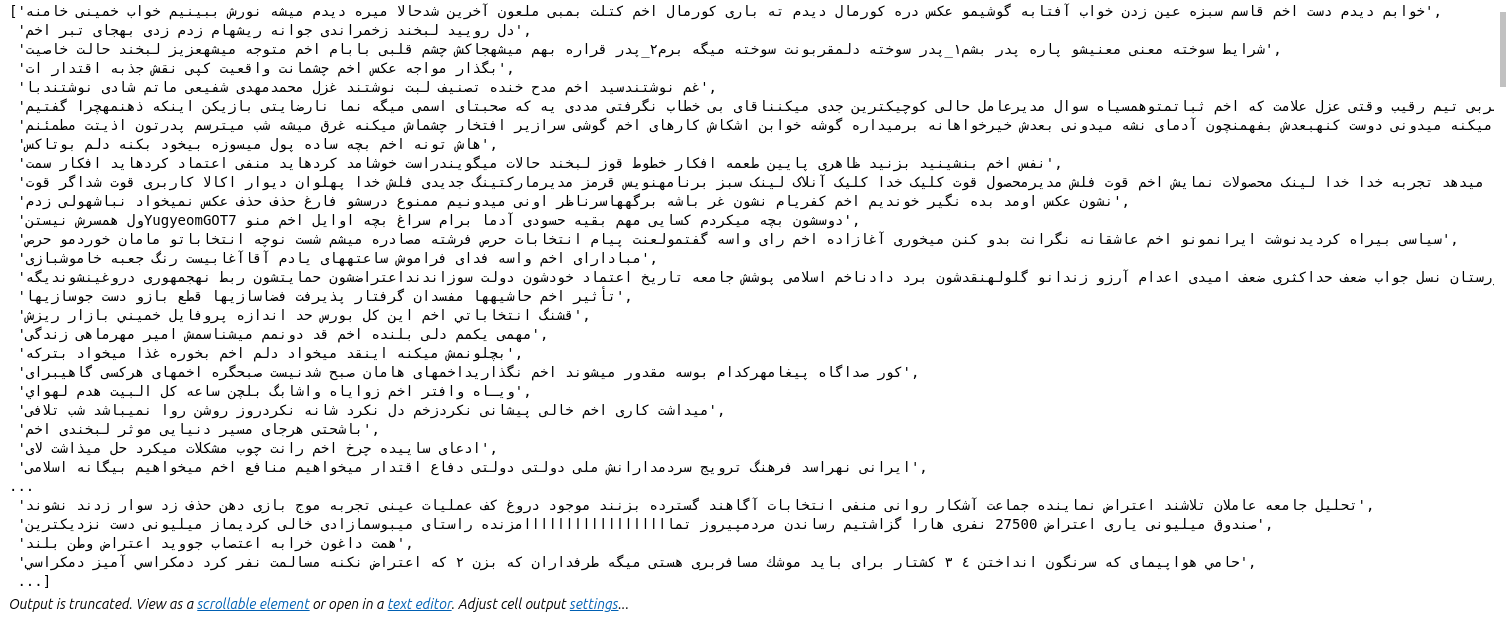
\includegraphics[width=0.5\linewidth]{pics/img7.png}
%		\end{minipage}
%		\hfill
%		\begin{minipage}[b]{0.3\textwidth}
%			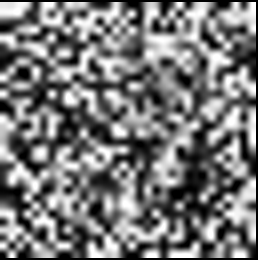
\includegraphics[width=0.5\linewidth]{pics/img8.png}
%		\end{minipage}
%		\hfill
%		\begin{minipage}[b]{0.3\textwidth}
%			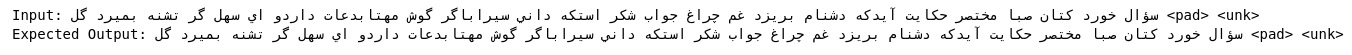
\includegraphics[width=0.5\linewidth]{pics/img9.png}
%		\end{minipage}
%		
%		\vspace{0.3cm}
%		
%		\begin{minipage}[b]{0.3\textwidth}
%			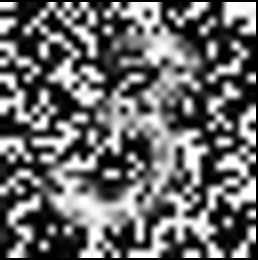
\includegraphics[width=0.5\linewidth]{pics/img10.png}
%		\end{minipage}
%		\hfill
%		\begin{minipage}[b]{0.3\textwidth}
%			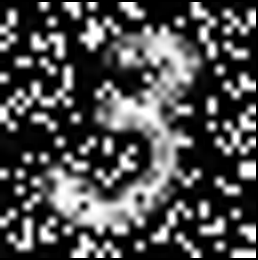
\includegraphics[width=0.5\linewidth]{pics/img11.png}
%		\end{minipage}
%		\hfill
%		\begin{minipage}[b]{0.3\textwidth}
%			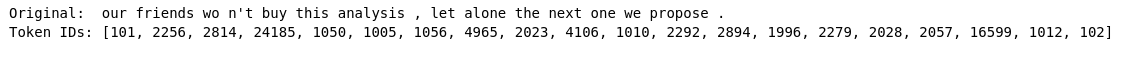
\includegraphics[width=0.5\linewidth]{pics/img12.png}
%		\end{minipage}
%		
%		\caption{خروجی‌های تولید شده در مرحله معکوس}
%	\end{figure}
%\end{center}
%
%
%
%
%
%\end{enumerate}
%
%
%
%
%
%
%
%
%
%
%
%
%
%
%
%
%
%
%
%
%
%
%
%
%
%
%
%
%
%
%
%
%
%
%
%
%
%%آیا تا کنون به روند عملکرد بهینه‌سازها فکر کرده‌اید؟ آیا می‌توان آن را یک شبکه‌ی بازرخدادی در نظر گرفت؟ در این پروژه هدف طراحی و پیاده‌سازی یک بهینه‌ساز می‌باشد. برای درک بهتر، توضیحات ریاضیاتی زیر داده می‌شود.
%%
%%
%%
%%روند یادگیری پارامترهای ($\theta$) یک شبکه عمیق ($f$) با الگوریتم های مرسوم نزول در راستای گرادیان (نظیر \lr{SGD}) را می‌توان به ازای ورودی‌های آموزشی $x$ بصورت رابطه‌ی (۱) در نظر گرفت:
%%
%%\begin{equation}
%%	\theta_{i+1} = \theta_i - \alpha \nabla f(x; \theta_i)
%%\end{equation}
%%
%%حال اگر فرض شود که به جای نرخ یادگیری ثابت $\alpha$ از یک تابع (شبکه‌ی عمیق) نظیر $g$ با پارامترهای قابل یادگیری $\phi$ استفاده کنیم، می‌توان رابطه‌ی (۱) را بصورت رابطه‌ی (۲) بازنویسی نمود:
%%
%%\begin{equation}
%%	\theta_{i+1} = \theta_i + g(\nabla f(x; \theta_i); \phi)
%%\end{equation}
%%
%%در نهایت می‌توان پارامتر $\theta_i$ را نیز به عنوان یک ورودی دیگر به $g$ در نظر گرفت و رابطه‌ی (۲) را نیز بصورت زیر بازنویسی کرد:
%%
%%\begin{equation}
%%	\theta_{i+1} = g(\nabla f(x; \theta_i), \theta_i; \phi)
%%\end{equation}
%%
%%حال می‌توان نتیجه گرفت که اگر تابع $g$ را یک شبکه‌ی بازرخدادی (نظیر \lr{LSTM} یا \lr{GRU}) در نظر گرفت، امکان ارئه‌ی یک بهینه‌ساز وجود دارد، که کل فرایند یاد شده را می‌توان با دو حلقه (بیرونی\footnote{\lr{Outer loop}} و درونی\footnote{\lr{Inner loop}}) انجام داد که معماری کلی آن در ادامه ضمیمه شده است. پیمایش یکبار حلقه‌ی بیرونی معادل است با یک تکرار (\lr{Epoch}) برای آموزش شبکه‌ی $g$ و پیمایش یکبار حلقه درونی معادل است با تولید یک داده آموزشی برای شبکه‌ی $g$.
%%
%%
%%
%%در این سوال هدف طراحی و پیاده سازی یک بهینه‌ساز بر اساس توضیحات فوق می‌باشد:
%%
%%\begin{enumerate}
%%	\item
%%مجموعه داده اول را به عنوان مجموعه آموزشی در نظر بگیرید، آن را نمایش داده و پس درهم سازی به ۵۰ زیر مجموعه تقسیم کنید بطوریکه در هر مجموعه داده از هر کلاس به تعداد برابر نمونه موجود باشد و انتخاب نمونه‌ها نیز با احتمال یکنواخت صورت گرفته باشد. حال، یک شبکه‌ی \lr{MLP} دلخواه طراحی نمایید و آن را $f$ بنامید که $f_1, f_2, \ldots$ شبکه‌های \lr{MLP} با معماری یکسان هستند و صرفا مقادیردهی اولیه‌ی آن‌ها هر بار متفاوت است.
%%	
%%	\begin{qsolve}
%%مجموعه داده ورودی (\texttt{dataset\_1.csv}) متشکل از نقاط \texttt{x} ،\texttt{y} و \texttt{label} ای است که جدا کننده دو کلاس داده‌ها است. ابعاد این دیتاست $(100000, 3)$ است.
%%	\end{qsolve}
%%	
%%	
%%	
%%	\begin{qsolve}
%%	
%%		\begin{center}
%%			\includegraphics*[width=0.4\linewidth]{pics/img1.png}
%%			\captionof{figure}{خروجی دیتاست \texttt{dataset\_1.csv}}
%%			\label{خروجی دیتاست ۱}
%%		\end{center}
%%		
%%		رسم گرافیکی دیتاست ورودی به‌صورت زیر است:
%%		
%%		\begin{center}
%%			\includegraphics*[width=0.5\linewidth]{pics/img2.png}
%%			\captionof{figure}{دیتاست \texttt{dataset\_1.csv}}
%%			\label{دیتاست ۱}
%%		\end{center}
%%		
%%		سپس طبق صورت مسئله،‌ دیتاست ورودی را به ۵۰ زیردیتاست تقسیم می‌کنیم. سایز زیردیتاست های تولید شده $(2000, 3)$ است. در ادامه خروجی این تقسیم دیتاست آورده شده است:
%%	\end{qsolve}
%%	
%%	
%%	\begin{qsolve}
%%		\begin{center}
%%			\includegraphics*[width=0.5\linewidth]{pics/img3.png}
%%			\captionof{figure}{زیردیتاست های تولید شده}
%%			\label{زیردیتاست ۱}
%%		\end{center}
%%		
%%		
%%		در ادامه شبکه ای \texttt{MLP} با مشخصات زیر تعریف شده است:
%%		\begin{itemize}
%%			\item تعداد نرون های ورودی:‌ ۲
%%			\item تعداد لایه‌های مخفی: ۲
%%			\item تعداد نرون‌های لایه مخفی اول: ۱۲۸
%%			\item تعداد نرون‌های لایه مخفی دوم: ۶۴
%%			\item تعداد نرون‌های خروجی: ۱
%%			\item تابع فعالساز: \texttt{ReLU}
%%		\end{itemize}
%%	\end{qsolve}
%%	
%%	
%%	
%%	
%%	\item 
%%یک شبکه‌ی بازرخدادی مبتنی بر \lr{GRU} طراحی نمایید و آن را $g$ بنامید که وظیفه‌ی آن بهینه‌سازی وزن‌های قابل یادگیری معماری $f$ برای هدف مورد نظر می‌باشد. با استفاده از ۵۰ زیر مجموعه‌ی ایجاد شده در قسمت قبل، شبکه‌ی $g$ را آموزش دهید. روند پیاده‌سازی آموزش، معماری طراحی شده و سایر جزئیات مورد نظر را در گزارش درج نمایید. توجه داشته باشید به ازای هر حلقه‌ی درونی (در هر حلقه‌ی بیرونی)، یک مقداردهی کاملا جدید برای شبکه‌ی $f$ صورت می‌گیرد. در هر زیر مجموعه نسبت آموزش به آزمون ۲:۸ است.
%%
%%
%%	\begin{qsolve}
%%	در این قسمت، بهینه‌سازی مبتنی بر شبکه بازرخدادی \texttt{GRU} با مشخصات زیر تعریف می‌کنیم:
%%		
%%		\begin{itemize}
%%			\item سایز ورودی: ۲
%%			\item سایز لایه مخفی: ۱۲۸
%%			\item سایز خروجی:‌ ۱
%%			\item نرخ یادگیری: ۰٫۰۰۱	
%%		\end{itemize}
%%		
%%		سپس شبکه $g$ را با زیرداده های بدست آورده آموزش می‌دهیم و به میانگین دقت و خطای زیر می‌رسیم:
%%		
%%		\begin{latin}
%%			\texttt{Average Accuracy: 49.99}\\
%%			\texttt{Average Error: 2.2704}
%%		\end{latin}
%%	\end{qsolve}
%%
%%
%%
%%
%%
%%
%%	\item
%%مجموعه داده‌ی دوم را نیز بارگذاری کرده و آن را نمایش دهید و تفاوت‌های آن را با مجموعه داده‌ی اول بیان کنید. حال آن را به ۳۰ زیر مجموعه همانند توضیحات قسمت ۱ تقسیم کنید. در نهایت، به ازای هر مجموعه داده، یک شبکه با معماری $f$ در نظر گرفته و با شبکه‌ی $g$ آن را بهینه‌سازی کنید. میانگین دقت و خطا را گزارش نمایید.
%%
%%
%%	\begin{qsolve}
%%در این قسمت مجموعه داده دوم (\texttt{dataset\_2.csv}) را می‌خوانیم و آن را نمایش می‌دهیم. این دو دیتاست در ظاهر شبیه‌به هم هستند اما ابعاد آنها با هم متفاوت است. 
%%
%%ابعاد دیتاست \texttt{dataset\_2.csv}، $(60000, 3)$ است.
%%
%%	\begin{center}
%%		\includegraphics*[width=0.4\linewidth]{pics/img4.png}
%%		\captionof{figure}{خروجی دیتاست \texttt{dataset\_2.csv}}
%%		\label{خروجی دیتاست ۲}
%%	\end{center}
%%	
%%	دیتاست \texttt{dataset\_2.csv} به‌صورت زیر رسم می‌شود:
%%	
%%	\begin{center}
%%		\includegraphics*[width=0.5\linewidth]{pics/img5.png}
%%		\captionof{figure}{دیتاست \texttt{dataset\_2.csv}}
%%		\label{دیتاست ۲}
%%	\end{center}
%%	\end{qsolve}
%%	
%%	
%%	
%%	\begin{qsolve}
%%		در ادامه مشابه با قسمت قبل، دیتاست را می‌بایست به تعدادی زیردیتاست تقسیم کنیم. در این قسمت دیتاست ورودی را به ۳۰ زیردیتاست تقسیم می‌کنیم. ابعاد هر زیردیتاست مشابه با قسمت قبل، $(2000, 3)$ می‌شود.
%%		
%%		در ادامه مشابه با قسمت قبل، سعی می‌کنیم با استفاده از بهینه‌ساز $g$ وزن‌های شبکه $f$ را این‌بار با استفاده از دیتاست \texttt{dataset\_2.csv} بهینه‌سازی کنیم.
%%		
%%		در این قسمت نیز، از همان تابع $g$ تعریف شده در قسمت قبل استفاده شده است. پس از انجام آموزش، مقدار میانگین خطا و دقت به‌صورت زیر بدست می‌آید:
%%		
%%		\begin{latin}
%%			\texttt{Average Accuracy for dataset\_2: 49.96}\\
%%			\texttt{Average Error for dataset\_2: 1.8790}
%%		\end{latin}
%%		
%%	\end{qsolve}
%%
%%
%%
%%	\item
%%\textbf{(اختیاری)} با مطالعه و تحقیق روشی ارائه دهید تا بتوان عملکرد بهینه‌ساز $g$ را بصورت کمی و کیفی ارزیابی نموده و همچنین بتوان آن را با بهینه‌ساز \lr{ADAM} مقایسه نمود.
%%
%%\end{enumerate}
%%
%%
%%\begin{qsolve}
%%برای ارزیابی بهینه‌ساز $g$ میانگین دقت و خطا یکی از معیار‌های کمی مناسب برای ارزیابی است. همچنین می‌توان همانند سایر بهینه‌ساز ها معیار های کمی دیگری مانند \lr{F1-score }، \lr{AUC-ROC} و ... را به کد اضافه نمود و بر اساس آنها نیز عملکرد بهینه‌ساز را ارزیابی کرد.
%%
%%همچنین برای مقایسه خروجی‌های بهینه‌سازی که ما نوشته ایم با بهینه‌سازی مانند \lr{Adam} می‌توان شبکه را دوبار با همین دیتاست‌ها یک بار با بهینه‌ساز $g$ و بار دیگر با بهینه‌ساز \lr{Adam} آموزش داد و سپس خروجی‌های آنها که شامل میانگین دقت، خطا، امتیاز \lr{F1} و ... است مقایسه کنیم.
%%
%%برای مقایسه کیفی نیز می‌توان از نمایش لصری توزیع داده‌های پیش‌بینی شده توسط هر دو بهینه‌ساز استفاده نمود.
%%
%%همچنین معیاری دیگر برای برای مقایسه، بررسی پایداری بهینه‌ساز نوشته شده توسط ما و بهینه‌ساز \lr{Adam} نسبت به تغییر پارامتر‌های ورودی شبکه و نرخ یادگیری است. مطلوب است بهینه‌ساز در برابر تغییرات پارامتر‌های ورودی شبکه نظیر نرخ یادگیری، تعداد \lr{Epoch} و ... کمترین میزان تغییر و نوسان را داشته باشد.
%%\end{qsolve}
%%
%%
%%
%%
%%
%%
%%
%%
%%
%%
%%
%%
%%
%%
%%
%%
%%
%%
%%
%%
%%
%%
%%
%%
%%
%%
%%
%%
%%
%%
%%
%%
%%
%%
%%
%%
%%
%%
%%
%%
%%
%%
%%
%%
%%
%%
%%%شبکه‌های عمیق از عدم تفسیر‌پذیری رنج می‌برند. تلاش برای حل این مشکل، دو ایده \lr{Deconvolutional} و \lr{Up-convolutional} مظرح شده است. بررسی کنید و توضیح دهید هرکدام از دو روش، به چه صورت منجر به تفسیرپذیری می‌شوند؟
%%%
%%%
%%%
%%%\begin{qsolve}
%%%	پیش از توضیح دادن این دو روش که چگونه به تفسیرپذیری کمک می‌کنند، ابتدا این دو روش را مختثرا توضیح می‌دهیم.
%%%	
%%%	
%%%	\begin{enumerate}
%%%		\item \textbf{شبکه \lr{Deconvolutional} یا \lr{Transposed convolutional layer}: }\\
%%%در لایه‌های کانولوشن ویژگی‌های مهم تصویر با استفاده از یک کرنل استخراج می‌شود و خروجی به عنوان \lr{Feature map} شناخته می‌شود. ابعاد تصویر (ممکن است) کاهش یابد و اطلاعات مهم تصویر حفظ می‌شود.
%%%
%%%
%%%	\begin{center}
%%%		\includegraphics*[width=0.6\linewidth]{pics/img4.png}
%%%		\captionof{figure}{لایه کانولوشن}
%%%		\label{لایه کانولوشن}
%%%	\end{center}
%%%	
%%%	
%%%	
%%%	لایه \lr{Deconvolution} دقیقا برعکس لایه‌های کانولوشنی عمل می‌کند. یعنی از یک \lr{Feature map} می‌توان به تصویر رسید. الگ.ریتم \lr{Deconv} با نگاشت نقشه‌های ویژگی‌ به فضای ورودی، این امکان را فراهم می‌کند 
%%%
%%%
%%%
%%%
%%%
%%%	
%%%	
%%%		\item \textbf{\lr{ :Up-Convolution}}
%%%لایه \lr{Up-convolution} نیز همانند \lr{Deconvolution} ابعاد ورودی را زیاد می‌کند و هدف آن تولید یک تصویر بزرگتر از ورودی آن است.
%%%
%%%	\begin{center}
%%%		\includegraphics*[width=0.6\linewidth]{pics/img5.png}
%%%		\captionof{figure}{لایه \lr{Up-convolution}}
%%%		\label{لایه آپ‌کانولوشن}
%%%	\end{center}
%%%	\end{enumerate}
%%%	
%%%	
%%%	در بسیاری از مراجه این دو تکنیک را معادل‌با هم می‌گیرند چرا که در هر دو روش هدف افزایش ابعاد ورودی است و این کار دقیقا برعکس کانولوشن انجام می‌شود.
%%%\end{qsolve}
%%%
%%%
%%%
%%%
%%%\begin{qsolve}
%%%	لایه \lr{Deconvolution} و \lr{Up-convolution}با نمایش نقشه‌های ویژگی به فضای ورودی، به ما امکان می‌دهد ببینیم چه نوع الگوهای ورودی نورون‌های خاصی را فعال می‌کنند. در \lr{Up-convolution} 
%%%\end{qsolve}
%%%
%%%
%%%
%%%
%%%\begin{latin}
%%%	\begin{thebibliography}{9}
%%%		\bibitem{ref1}
%%%		Durall R, Keuper M, Keuper J. Watch your up-convolution: Cnn based generative deep neural networks are failing to reproduce spectral distributions. InProceedings of the IEEE/CVF conference on computer vision and pattern recognition 2020 (pp. 7890-7899).
%%%		
%%%	\end{thebibliography} 
%%%\end{latin}
